\documentclass[12pt]{article}
\usepackage{lingmacros}
\usepackage{tree-dvips}
\usepackage{titlesec}
\usepackage{amsmath}
\usepackage{hyperref}
\usepackage{graphicx}
\usepackage{array}
\usepackage{makecell}

\renewcommand\theadalign{bc}
\renewcommand\theadfont{\bfseries}

\hypersetup{
    colorlinks,
    citecolor=black,
    filecolor=black,
    linkcolor=black,
    urlcolor=black
}


\setcounter{secnumdepth}{4}
\begin{document}
\title{%
  'PowerShare' project document \\
  \large High Tech Entrepreneurship \\
  Politecnico di Milano \\
}
\graphicspath{ {./images/} }
\maketitle
\tableofcontents

\newpage
    \section{Executive Summary}
    \section{The Team}
        \subsection{Management Profile}
        \subsection{Why we are a winning team}
    \section{The Business Model}
        \subsection{Value Proposition, Vision, Mission and Values}
        \subsection{Customer Segments}
        \subsection{Marketing Plan}
        \subsection{Key resources and activities}
    \newpage
    \section{External Environment}
        In the following analysis, we focused on three main markets. In the first section, 
        the Chinese market will be discussed: it is the only market in which the power bank sharing business is quite developed. 
        Because of that, we think that it represents an example of the possible outcome of our business. 
        Furthermore, the companies active in the Chinese market are well established and have been active for 5 years. 
        Therefore, they may represent a possible new entrant in the European or Italian market.  
        In the second paragraph, we decided to focus on the Italian market, which is much less developed and still in growing.  
        
        \subsection{Market analysis and key trends}
            \subsubsection{China Market}
            The power bank sharing is a well-established business in China, 
            and in the last years the Chinese market has been growing fast. 
            The trend is positive and growing. In 2018 there were an average number of users of 1,16 Million, 
            reaching 1,3 Million users in the half of 2019 and it is expected to reach 400 Million users by the end of 2020. 
            \begin{figure}[h]
                \centering
                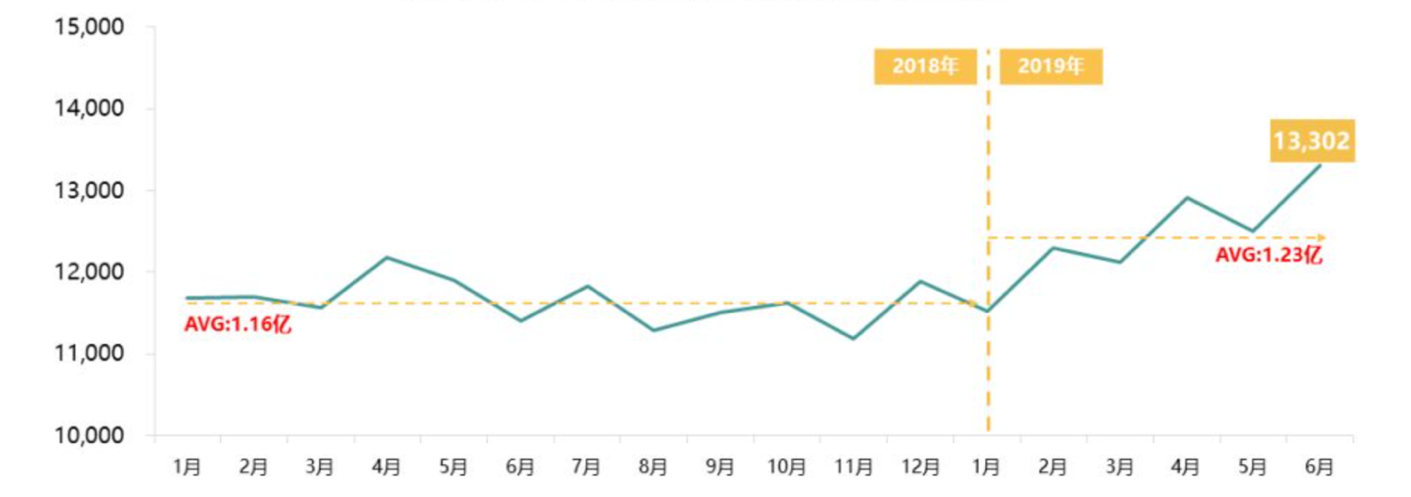
\includegraphics[width=1\textwidth]{china_graph}
                \caption{Number of reached users per month in China market}
            \end{figure}
            \newline
            The shared power bank stations penetrated in several mainstream consumers scenarios. 
            Power bank sharing companies can be found mainly in shopping malls, shopping centers, restaurant and bars and public transport stations. 
            
            \begin{figure}[h]
                \centering
                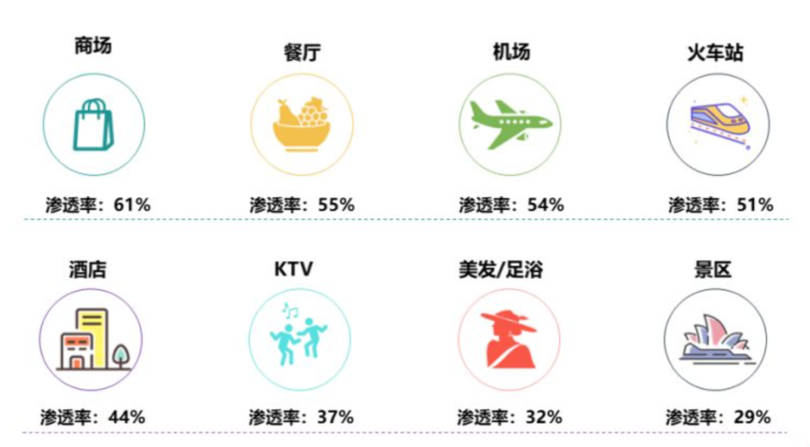
\includegraphics[width=0.75\textwidth]{china_locations}
                \caption{Consumer scenarios}
            \end{figure}            
            Nowadays, a lot of companies and startups are active in the power bank sharing market. 
            Within it, we can identify three market leaders of same dimension, which together control more than 80\% of the total market. 
            These companies are known as Jidian, Xiaodian and Energy Monster. This companies will be further discussed in the competitors' section. 
            The share of the shared charging market in 2019 (unit: \%). 
            \begin{figure}[h]
                \centering
                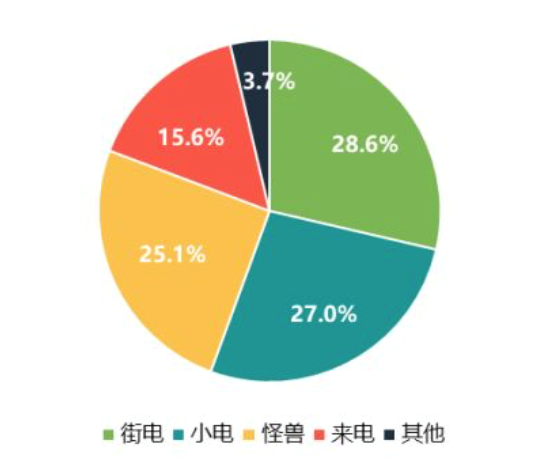
\includegraphics[width=0.75\textwidth]{china_pie_chart}
                \caption{Consumer scenarios}
            \end{figure}
            According to market research, nearly 70\% of the power bank service users are aged 30 and below. 
            Instead, there is no distinction related to the mobile phones operative system: 
            among the power bank users the proposition of Android users and Apple users is the same. 
            Similarly, also in the behavior (monthly usage frequency and average usage time) 
            it seems not to be a relevant difference between the two categories of users. 
            \begin{figure}[h]
                \centering
                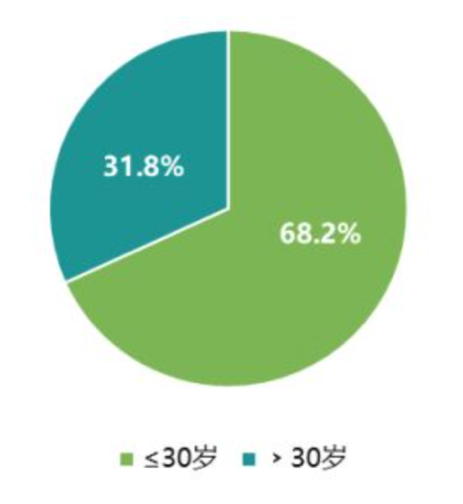
\includegraphics[width=0.75\textwidth]{china_pie_chart_ages}
                \caption{age characteristics of shared charging users in 2019}
            \end{figure}
            Among the shared charging users in 2019, the proportion of Android users and Apple users is quite the same
            \begin{figure}[h]
                \centering
                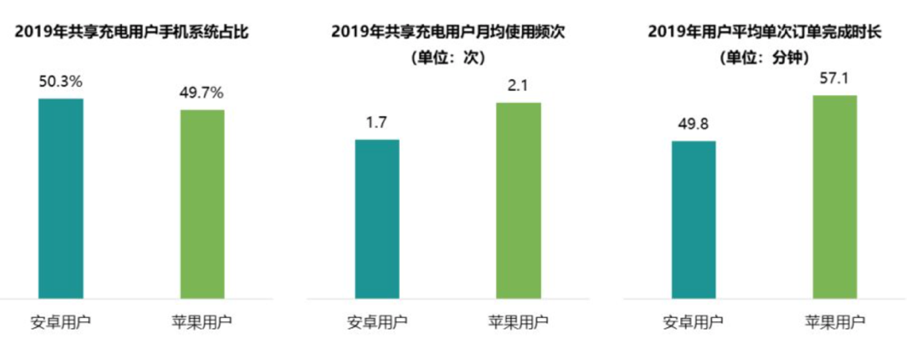
\includegraphics[width=0.75\textwidth]{china_usage_chart}
                \caption{from left: Proportion of shared charging users' mobile phone systems in 2019; 
                Average monthly usage frequency of shared charging users in 2019; 
                Average user completion time of single order in 2019 (unit: minutes)}
            \end{figure}
            \newpage
            Remarks: The monthly use frequency of this page and the length of time for a single order to complete the show, 
            statistics of high frequency make Ming users, that is, users who have used the shared charging treasure more than 50 times in the past year.
            The shared charging market has entered the stage of upgrading and development, and the future is expected
            \newline
                Now: 
                \begin{itemize}
                    \item Changes in the current status of deposit leasing to credit leasing usage patterns, 
                    improving user convenience and accelerating the expansion of user scale; 
                    \item The use price has increased from 1 yuan per hour to 2 yuan per hour, further reducing operating costs; 
                    \item The cooperation model with offline merchants has been upgraded to income 
                    Divided to reduce operating costs while accelerating the offline penetration rate;   
                \end{itemize}
                \newpage
                In the future:
                \begin{itemize}
                    \item we will further increase the penetration rate and reach more users by covering more scenarios; 
                    \item Shared charging manufacturers actively explore multiple business models to ensure profit while reducing user usage costs; 
                    tration rate and reach more users by covering more scenarios;
                    \item grasp market changes, improve user experience, and embrace 5G.
                \end{itemize}
            \subsubsection{Italian Market}
                The Italian (and European) market is almost not existing today. 
                Several companies were born in the last years, on the flow of the Chinese model. 
                However almost all of them are still in a seed stage and concentrated in a small area or in a single country. 
                A couple of them are expanding and trying to enter other countries’ markets.
                As in the other countries, the Italian power bank sharing is not developed at all. 
                However, looking at the Chinese example, at general spreading of the sharing economy and at the future development of the technology,
                we believe that this demand can be created. According to a survey conducted among an ensemble of nearly 400 people, 84\% 
                perceive their smartphone running-out-of-battery as a problem. Almost 30\% of the interviewed face this problem more or at least
                once a week without the possibility to plug it. Some external factors are relevant and contributes to the adoption of a power bank sharing service. 
                \newline
                factors: Covid
            \paragraph*{Technological factors}
                The arrival of 5G era will increase the power consumption and therefore the request of power banks. 
                Furthermore, since more and more devices will be part of the IoT and connected, 
                probably the necessity of charging will not me limited to smartphones and tablets anymore. 

            \paragraph*{Social factors} 
                The increased number of users of a sharing service and therefore the already established “sharing mentality” among people, 
                especially regarding who lives or works in a big city.

            \paragraph*{Environmental factors} 
                The increasing environmental consciousness will positively contribute to the adoption of such a service, 
                since it makes more efficient the power bank usage and reduces the numbers of unused batteries. 
                Considering the total Italian market, we expect to have X of potential users and a market of X value. Regarding the city of Milan itself…. 

            \paragraph*{Internal rivalry}
                The Italian power bank sharing demand began to be shaped in 2019 and the market is characterized by a few numbers of players: 
                only three companies are currently working in that market. 
                These companies are Mobbi (born in febbruary 2020), Caricami and Beepower. 
                \newline All of them are in a seed stage and their dimension is small. 
                In particular Mobbi is present in the center of Milan with around 200 stations, Caricami has 33 and Beepower only 4. 
                The latter is also present in Livorno, Riccione and Firenze but the total number of stations does not go beyond 10. 
                The market is promising and growing. None of their brand seems to be strong, therefore it is reasonable to assume that the customer loyalty towards is low. 
                Chimpy is….

            \paragraph*{Possible new entrants}
                The market is newborn and therefore attractive. 
                There are no particular regulations that obstacles the entrance in this market. 
                It requires a considerable initial investment, since it is important to scale and reach an economy of scale that the already established competitors will have. 
                However, after a detailed analysis of the provider around the Europe and the World, 
                a few players are big and established enough to be considered sufficiently threatening. 
                Regarding Europe, only Charged Up seems to represent a possible threat, but since its plan is to enter Spanish, French, German and Dutch markets, 
                it is unlikely that it will enter also the Italian market in the short term. 
                Looking at the Chinese market, the companies that most likely will expand in the Italian market may be the three bigs: Jiedian, Xiaodian and Energy Monster. 
                It is not unlikely that a Chinese sharing company enters an Italian market, since it already happened with Mobike. 
                Therefore, they may represent a possible threat.

            \paragraph*{Possible Substitutes}
                Possible substitutes are shops that sells power banks and bar or places that allow you to plug your device. 
                The former has definitely a high switching cost and it is less attractive since you will have to carry it around. 
                The latter may be less attractive too, since you do not have the same flexibility you would have with a power bank (You have to stay in a place). 
                Furthermore, there is not great availability of places where you can plug your device. 
                It is reasonable not to consider these substitutes as a threat.
                The market is not mature yet and the demand has already to be shaped. 
                The competition is present, but low, since the few companies active in this sector are still in a seed stage. 
                Possible, but limited threats may be represented by the Chinese companies. 
                Therefore, it is reasonable to conclude that this market represents a good opportunity to begin a business.

            \subsection{Competitors' analysis}
            \begin{table}[h!]
                \begin{center}
                  \caption{Multirow table.}
                  \label{tab:table1}
                  \begin{tabular}{|c|c|c|c|c|c|c|c|}
                    \thead{Feature} & \thead{Mobbi} & \thead{Caricami} & \thead{Beepower} & \thead{ChargedUp} \\
                    \hline
                    \makecell{Multiple connector}                 & Yes & Yes & Yes & No & Yes \\
                    \hline
                    Fast Charge                          & Yes & Yes & Portable & Portable & Portable \\
                    \hline
                    Design                               & Yes & No  & No & No & No \\
                    \hline
                    Capacity                             & 5000mAh & 5000mAh & 5000mAh & 5000mAh & No \\
                    \hline
                    Home charging                        & No  & Probable & No & Probable & Yes \\
                    \hline
                    Deposit                              & No  & Yes (max 10€) & Yes (10€) & Yes & Unknown \\
                    \hline
                    Subscription                         & No  & Yes & Yes & Yes (premium) & Yes \\
                    \hline
                    \makecell{Apple Pay GPay other platforms}       & Apple Pay & No & Satispay & No & No \\
                    \hline
                    \makecell{Renting with dead smartphone}         & Unknown & Unknown & Unknown & Unknown & Unknown \\
                    \hline
                    Events                               & Unknown & Yes & Yes & No & Yes \\
                    \hline
                    \makecell{Multiple charge at same time}         & Unknown & Yes & Probable & No & No \\
                    \hline
                    \makecell{Booking in advance}                   & No & No & No & No & No \\
                    \hline
                    Wireless                             & No & No & Yes & No & No \\
                    \hline
                    Public transport            & No & No & No & No & No \\
                    \hline
                    University                  & No & No & No & unknown & No \\
                    \hline
                    Eco friendly                         & No & No & Yes & Yes & Yes \\
                    \hline
                  \end{tabular}
                \end{center}
              \end{table}
        \subsection{Competitive advatages of the business model}
    \section{Sketch of the Business Model Canvas}
    \section{Sketch of the financial analysis (including funding requirements)}
    \section{Roadmap}

\end{document}